% Created by tikzDevice version 0.12.6 on 2025-12-26 04:00:37
% !TEX encoding = UTF-8 Unicode
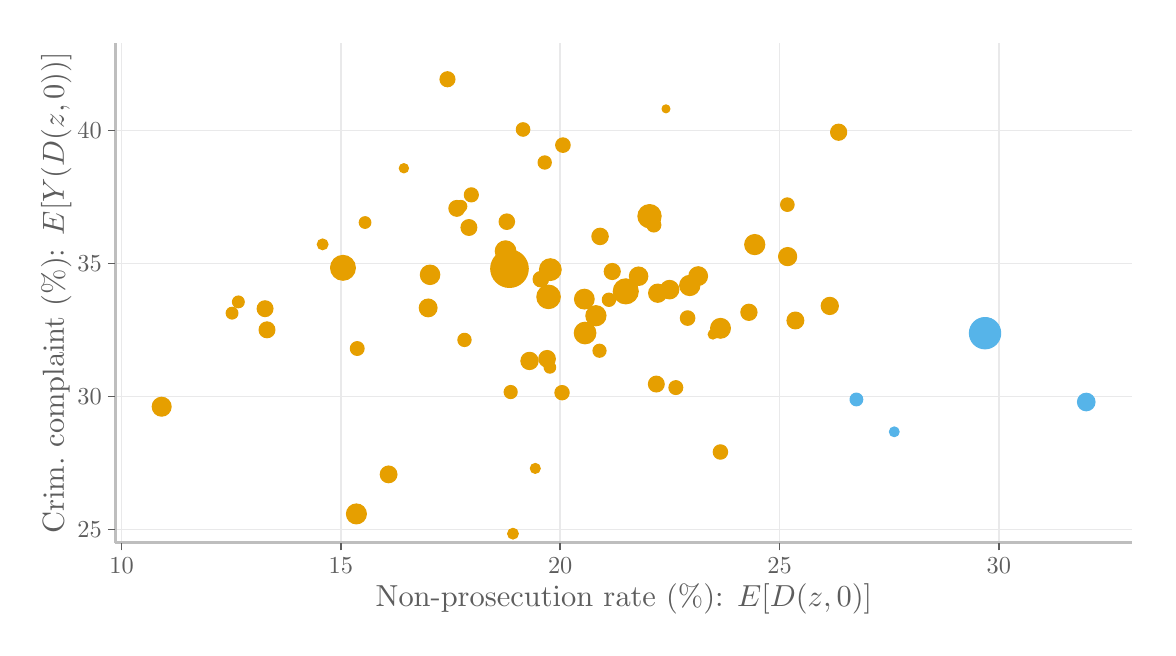
\begin{tikzpicture}[x=1pt,y=1pt]
\definecolor{fillColor}{RGB}{255,255,255}
\path[use as bounding box,fill=fillColor,fill opacity=0.00] (0,0) rectangle (404.71,216.81);
\begin{scope}
\path[clip] (  0.00,  0.00) rectangle (404.71,216.81);
\definecolor{drawColor}{RGB}{255,255,255}
\definecolor{fillColor}{RGB}{255,255,255}

\path[draw=drawColor,line width= 0.6pt,line join=round,line cap=round,fill=fillColor] (  0.00,  0.00) rectangle (404.71,216.81);
\end{scope}
\begin{scope}
\path[clip] ( 31.71, 30.69) rectangle (399.21,211.31);
\definecolor{fillColor}{RGB}{255,255,255}

\path[fill=fillColor] ( 31.71, 30.69) rectangle (399.21,211.31);
\definecolor{drawColor}{RGB}{233,233,234}

\path[draw=drawColor,line width= 0.6pt,line join=round] ( 31.71, 35.46) --
	(399.21, 35.46);

\path[draw=drawColor,line width= 0.6pt,line join=round] ( 31.71, 83.54) --
	(399.21, 83.54);

\path[draw=drawColor,line width= 0.6pt,line join=round] ( 31.71,131.62) --
	(399.21,131.62);

\path[draw=drawColor,line width= 0.6pt,line join=round] ( 31.71,179.70) --
	(399.21,179.70);

\path[draw=drawColor,line width= 0.6pt,line join=round] ( 33.92, 30.69) --
	( 33.92,211.31);

\path[draw=drawColor,line width= 0.6pt,line join=round] (113.18, 30.69) --
	(113.18,211.31);

\path[draw=drawColor,line width= 0.6pt,line join=round] (192.44, 30.69) --
	(192.44,211.31);

\path[draw=drawColor,line width= 0.6pt,line join=round] (271.70, 30.69) --
	(271.70,211.31);

\path[draw=drawColor,line width= 0.6pt,line join=round] (350.96, 30.69) --
	(350.96,211.31);
\definecolor{drawColor}{RGB}{230,159,0}
\definecolor{fillColor}{RGB}{230,159,0}

\path[draw=drawColor,line width= 0.4pt,line join=round,line cap=round,fill=fillColor] (186.83,168.09) circle (  2.39);

\path[draw=drawColor,line width= 0.4pt,line join=round,line cap=round,fill=fillColor] (185.43,125.92) circle (  2.80);

\path[draw=drawColor,line width= 0.4pt,line join=round,line cap=round,fill=fillColor] (187.68, 97.16) circle (  2.99);

\path[draw=drawColor,line width= 0.4pt,line join=round,line cap=round,fill=fillColor] (274.61,134.09) circle (  3.27);

\path[draw=drawColor,line width= 0.4pt,line join=round,line cap=round,fill=fillColor] (193.41,174.37) circle (  2.62);

\path[draw=drawColor,line width= 0.4pt,line join=round,line cap=round,fill=fillColor] (121.91,146.40) circle (  2.10);

\path[draw=drawColor,line width= 0.4pt,line join=round,line cap=round,fill=fillColor] (210.04,118.49) circle (  2.40);

\path[draw=drawColor,line width= 0.4pt,line join=round,line cap=round,fill=fillColor] (277.41,111.00) circle (  3.04);

\path[draw=drawColor,line width= 0.4pt,line join=round,line cap=round,fill=fillColor] (211.23,128.70) circle (  2.90);

\path[draw=drawColor,line width= 0.4pt,line join=round,line cap=round,fill=fillColor] (159.44,144.60) circle (  2.86);

\path[draw=drawColor,line width= 0.4pt,line join=round,line cap=round,fill=fillColor] (144.71,115.54) circle (  3.21);

\path[draw=drawColor,line width= 0.4pt,line join=round,line cap=round,fill=fillColor] (201.15,118.72) circle (  3.56);

\path[draw=drawColor,line width= 0.4pt,line join=round,line cap=round,fill=fillColor] (130.42, 55.39) circle (  3.02);

\path[draw=drawColor,line width= 0.4pt,line join=round,line cap=round,fill=fillColor] (205.33,112.72) circle (  3.64);

\path[draw=drawColor,line width= 0.4pt,line join=round,line cap=round,fill=fillColor] (151.69,198.17) circle (  2.71);

\path[draw=drawColor,line width= 0.4pt,line join=round,line cap=round,fill=fillColor] (220.76,126.99) circle (  3.33);

\path[draw=drawColor,line width= 0.4pt,line join=round,line cap=round,fill=fillColor] (188.70, 94.05) circle (  2.08);

\path[draw=drawColor,line width= 0.4pt,line join=round,line cap=round,fill=fillColor] (227.66,120.86) circle (  3.29);

\path[draw=drawColor,line width= 0.4pt,line join=round,line cap=round,fill=fillColor] (216.12,121.53) circle (  4.52);

\path[draw=drawColor,line width= 0.4pt,line join=round,line cap=round,fill=fillColor] (118.79, 41.10) circle (  3.60);

\path[draw=drawColor,line width= 0.4pt,line join=round,line cap=round,fill=fillColor] (106.58,138.51) circle (  1.95);

\path[draw=drawColor,line width= 0.4pt,line join=round,line cap=round,fill=fillColor] (201.41,106.47) circle (  3.90);

\path[draw=drawColor,line width= 0.4pt,line join=round,line cap=round,fill=fillColor] (135.94,166.01) circle (  1.67);
\definecolor{drawColor}{RGB}{86,180,233}
\definecolor{fillColor}{RGB}{86,180,233}

\path[draw=drawColor,line width= 0.4pt,line join=round,line cap=round,fill=fillColor] (299.46, 82.46) circle (  2.30);
\definecolor{drawColor}{RGB}{230,159,0}
\definecolor{fillColor}{RGB}{230,159,0}

\path[draw=drawColor,line width= 0.4pt,line join=round,line cap=round,fill=fillColor] ( 48.42, 79.84) circle (  3.42);

\path[draw=drawColor,line width= 0.4pt,line join=round,line cap=round,fill=fillColor] (172.69,136.05) circle (  3.73);

\path[draw=drawColor,line width= 0.4pt,line join=round,line cap=round,fill=fillColor] (173.14,146.70) circle (  2.79);

\path[draw=drawColor,line width= 0.4pt,line join=round,line cap=round,fill=fillColor] (242.28,127.04) circle (  3.38);

\path[draw=drawColor,line width= 0.4pt,line join=round,line cap=round,fill=fillColor] (262.72,138.43) circle (  3.63);

\path[draw=drawColor,line width= 0.4pt,line join=round,line cap=round,fill=fillColor] (250.35,108.17) circle (  3.58);

\path[draw=drawColor,line width= 0.4pt,line join=round,line cap=round,fill=fillColor] (238.46,111.87) circle (  2.62);

\path[draw=drawColor,line width= 0.4pt,line join=round,line cap=round,fill=fillColor] (113.93,130.03) circle (  4.49);

\path[draw=drawColor,line width= 0.4pt,line join=round,line cap=round,fill=fillColor] (250.32, 63.48) circle (  2.60);

\path[draw=drawColor,line width= 0.4pt,line join=round,line cap=round,fill=fillColor] (289.84,116.26) circle (  3.10);

\path[draw=drawColor,line width= 0.4pt,line join=round,line cap=round,fill=fillColor] (224.70,148.69) circle (  4.20);
\definecolor{drawColor}{RGB}{86,180,233}
\definecolor{fillColor}{RGB}{86,180,233}

\path[draw=drawColor,line width= 0.4pt,line join=round,line cap=round,fill=fillColor] (382.51, 81.54) circle (  3.17);
\definecolor{drawColor}{RGB}{230,159,0}
\definecolor{fillColor}{RGB}{230,159,0}

\path[draw=drawColor,line width= 0.4pt,line join=round,line cap=round,fill=fillColor] (193.09, 84.91) circle (  2.58);

\path[draw=drawColor,line width= 0.4pt,line join=round,line cap=round,fill=fillColor] (206.83,141.38) circle (  2.96);

\path[draw=drawColor,line width= 0.4pt,line join=round,line cap=round,fill=fillColor] (183.42, 57.55) circle (  1.80);

\path[draw=drawColor,line width= 0.4pt,line join=round,line cap=round,fill=fillColor] (247.60,106.00) circle (  1.71);

\path[draw=drawColor,line width= 0.4pt,line join=round,line cap=round,fill=fillColor] ( 85.78,115.26) circle (  2.86);

\path[draw=drawColor,line width= 0.4pt,line join=round,line cap=round,fill=fillColor] (226.26,145.52) circle (  2.54);

\path[draw=drawColor,line width= 0.4pt,line join=round,line cap=round,fill=fillColor] (160.31,156.40) circle (  2.54);

\path[draw=drawColor,line width= 0.4pt,line join=round,line cap=round,fill=fillColor] (231.95,122.15) circle (  3.34);

\path[draw=drawColor,line width= 0.4pt,line join=round,line cap=round,fill=fillColor] (274.51,152.86) circle (  2.44);

\path[draw=drawColor,line width= 0.4pt,line join=round,line cap=round,fill=fillColor] (188.87,129.38) circle (  3.92);

\path[draw=drawColor,line width= 0.4pt,line join=round,line cap=round,fill=fillColor] (188.21,119.53) circle (  4.24);

\path[draw=drawColor,line width= 0.4pt,line join=round,line cap=round,fill=fillColor] (181.34, 96.38) circle (  3.12);

\path[draw=drawColor,line width= 0.4pt,line join=round,line cap=round,fill=fillColor] ( 76.13,117.71) circle (  2.13);

\path[draw=drawColor,line width= 0.4pt,line join=round,line cap=round,fill=fillColor] (174.53, 85.14) circle (  2.36);

\path[draw=drawColor,line width= 0.4pt,line join=round,line cap=round,fill=fillColor] ( 86.48,107.62) circle (  2.87);

\path[draw=drawColor,line width= 0.4pt,line join=round,line cap=round,fill=fillColor] (179.00,180.02) circle (  2.44);

\path[draw=drawColor,line width= 0.4pt,line join=round,line cap=round,fill=fillColor] (230.65,187.48) circle (  1.43);

\path[draw=drawColor,line width= 0.4pt,line join=round,line cap=round,fill=fillColor] (175.36, 33.97) circle (  1.94);

\path[draw=drawColor,line width= 0.4pt,line join=round,line cap=round,fill=fillColor] (227.16, 88.03) circle (  2.86);

\path[draw=drawColor,line width= 0.4pt,line join=round,line cap=round,fill=fillColor] (157.84,103.98) circle (  2.39);

\path[draw=drawColor,line width= 0.4pt,line join=round,line cap=round,fill=fillColor] (234.21, 86.76) circle (  2.50);

\path[draw=drawColor,line width= 0.4pt,line join=round,line cap=round,fill=fillColor] ( 73.85,113.65) circle (  2.13);
\definecolor{drawColor}{RGB}{86,180,233}
\definecolor{fillColor}{RGB}{86,180,233}

\path[draw=drawColor,line width= 0.4pt,line join=round,line cap=round,fill=fillColor] (313.14, 70.77) circle (  1.77);
\definecolor{drawColor}{RGB}{230,159,0}
\definecolor{fillColor}{RGB}{230,159,0}

\path[draw=drawColor,line width= 0.4pt,line join=round,line cap=round,fill=fillColor] (239.24,123.65) circle (  3.65);

\path[draw=drawColor,line width= 0.4pt,line join=round,line cap=round,fill=fillColor] (155.06,151.51) circle (  2.86);

\path[draw=drawColor,line width= 0.4pt,line join=round,line cap=round,fill=fillColor] (156.57,152.27) circle (  2.10);

\path[draw=drawColor,line width= 0.4pt,line join=round,line cap=round,fill=fillColor] (206.63,100.07) circle (  2.36);

\path[draw=drawColor,line width= 0.4pt,line join=round,line cap=round,fill=fillColor] (119.08,100.87) circle (  2.49);

\path[draw=drawColor,line width= 0.4pt,line join=round,line cap=round,fill=fillColor] (293.04,179.03) circle (  2.91);

\path[draw=drawColor,line width= 0.4pt,line join=round,line cap=round,fill=fillColor] (145.40,127.51) circle (  3.51);

\path[draw=drawColor,line width= 0.4pt,line join=round,line cap=round,fill=fillColor] (260.62,113.96) circle (  2.92);
\definecolor{drawColor}{RGB}{86,180,233}
\definecolor{fillColor}{RGB}{86,180,233}

\path[draw=drawColor,line width= 0.4pt,line join=round,line cap=round,fill=fillColor] (345.94,106.41) circle (  5.65);
\definecolor{drawColor}{RGB}{230,159,0}
\definecolor{fillColor}{RGB}{230,159,0}

\path[draw=drawColor,line width= 0.4pt,line join=round,line cap=round,fill=fillColor] (174.10,129.72) circle (  6.78);
\end{scope}
\begin{scope}
\path[clip] (  0.00,  0.00) rectangle (404.71,216.81);
\definecolor{drawColor}{RGB}{190,190,190}

\path[draw=drawColor,line width= 1.1pt,line join=round] ( 31.71, 30.69) --
	( 31.71,211.31);
\end{scope}
\begin{scope}
\path[clip] (  0.00,  0.00) rectangle (404.71,216.81);
\definecolor{drawColor}{RGB}{93,93,93}

\node[text=drawColor,anchor=base east,inner sep=0pt, outer sep=0pt, scale=  0.88] at ( 26.76, 32.43) {25};

\node[text=drawColor,anchor=base east,inner sep=0pt, outer sep=0pt, scale=  0.88] at ( 26.76, 80.51) {30};

\node[text=drawColor,anchor=base east,inner sep=0pt, outer sep=0pt, scale=  0.88] at ( 26.76,128.59) {35};

\node[text=drawColor,anchor=base east,inner sep=0pt, outer sep=0pt, scale=  0.88] at ( 26.76,176.67) {40};
\end{scope}
\begin{scope}
\path[clip] (  0.00,  0.00) rectangle (404.71,216.81);
\definecolor{drawColor}{RGB}{93,93,93}

\path[draw=drawColor,line width= 0.6pt,line join=round] ( 28.96, 35.46) --
	( 31.71, 35.46);

\path[draw=drawColor,line width= 0.6pt,line join=round] ( 28.96, 83.54) --
	( 31.71, 83.54);

\path[draw=drawColor,line width= 0.6pt,line join=round] ( 28.96,131.62) --
	( 31.71,131.62);

\path[draw=drawColor,line width= 0.6pt,line join=round] ( 28.96,179.70) --
	( 31.71,179.70);
\end{scope}
\begin{scope}
\path[clip] (  0.00,  0.00) rectangle (404.71,216.81);
\definecolor{drawColor}{RGB}{190,190,190}

\path[draw=drawColor,line width= 1.1pt,line join=round] ( 31.71, 30.69) --
	(399.21, 30.69);
\end{scope}
\begin{scope}
\path[clip] (  0.00,  0.00) rectangle (404.71,216.81);
\definecolor{drawColor}{RGB}{93,93,93}

\path[draw=drawColor,line width= 0.6pt,line join=round] ( 33.92, 27.94) --
	( 33.92, 30.69);

\path[draw=drawColor,line width= 0.6pt,line join=round] (113.18, 27.94) --
	(113.18, 30.69);

\path[draw=drawColor,line width= 0.6pt,line join=round] (192.44, 27.94) --
	(192.44, 30.69);

\path[draw=drawColor,line width= 0.6pt,line join=round] (271.70, 27.94) --
	(271.70, 30.69);

\path[draw=drawColor,line width= 0.6pt,line join=round] (350.96, 27.94) --
	(350.96, 30.69);
\end{scope}
\begin{scope}
\path[clip] (  0.00,  0.00) rectangle (404.71,216.81);
\definecolor{drawColor}{RGB}{93,93,93}

\node[text=drawColor,anchor=base,inner sep=0pt, outer sep=0pt, scale=  0.88] at ( 33.92, 19.68) {10};

\node[text=drawColor,anchor=base,inner sep=0pt, outer sep=0pt, scale=  0.88] at (113.18, 19.68) {15};

\node[text=drawColor,anchor=base,inner sep=0pt, outer sep=0pt, scale=  0.88] at (192.44, 19.68) {20};

\node[text=drawColor,anchor=base,inner sep=0pt, outer sep=0pt, scale=  0.88] at (271.70, 19.68) {25};

\node[text=drawColor,anchor=base,inner sep=0pt, outer sep=0pt, scale=  0.88] at (350.96, 19.68) {30};
\end{scope}
\begin{scope}
\path[clip] (  0.00,  0.00) rectangle (404.71,216.81);
\definecolor{drawColor}{RGB}{93,93,93}

\node[text=drawColor,anchor=base,inner sep=0pt, outer sep=0pt, scale=  1.10] at (215.46,  7.64) {Non-prosecution rate (\%): $E[D(z, 0)]$};
\end{scope}
\begin{scope}
\path[clip] (  0.00,  0.00) rectangle (404.71,216.81);
\definecolor{drawColor}{RGB}{93,93,93}

\node[text=drawColor,rotate= 90.00,anchor=base,inner sep=0pt, outer sep=0pt, scale=  1.10] at ( 13.08,121.00) {Crim.~complaint (\%): $E[Y(D(z, 0))]$};
\end{scope}
\end{tikzpicture}
